%!TEX root = Manuscrit.tex
\chapter{Généralisation}
\label{chap:generalisation}
%\citationChap{The purpose of computing is insight, not numbers.}{Richard Hamming}
\minitoc

\chapsummary{%

}

\newpage

\section{Cas des données limitées}

\subsection{Apprentissage par transfert}

VEDAI -> Potsdam/Christchurch

Potsdam <-> Vaihingen

Différences de radiométrie, de résolutions

\subsection{Génération de données synthétiques}

Comme nous l'avons vu dans le~\cref{chap:extension}, les acquisitions hyperspectrales contiennent généralement peu d'exemples d'apprentissage compte-tenu de la rareté des annotations et de la faible résolution des imageurs.

Une solution consiste à augmenter les données de façon artificielle. En particulier, les \gls{GAN} forment une famille de modèles génératifs utilisant plusieurs réseaux profonds entraînés en concurrence.

L'augmentation de données consiste à introduire des échantillons synthétiques afin d'enrichir un jeu d'apprentissage statistique~\cite{dyk_art_2012}. C'est une pratique particulièrement courante pour l'entraînement des \gls{CNN} depuis l'article séminal de~\citet{krizhevsky_imagenet_2012} afin d'éviter le surapprentissage. Dans un contexte de classification de données hyperspectrales, la rareté des échantillons annotés rend l'augmentation de données d'autant plus attrayante. Cependant, les travaux récents appliquant des \gls{CNN} 3D à la classification de telles images~\cite{chen_deep_2016,makantasis_deep_2015,slavkovikj_hyperspectral_2015,lee_contextual_2016} se sont bornés à des jeux de données de petite taille ne permettant pas d'exploiter au mieux les représentations apprises par les réseaux profonds.

Récemment, certains travaux ont commencé à étudier les possibilités d'enrichir artificiellement les jeux de données hyperspectraux publics. Par exemple, \cite{windrim_hyperspectral_2016} ont proposé un modèle permettant de simuler des spectres sous différentes conditions d'illuminations. \cite{acquarelli_convolutional_2017} ont quant à eux proposé une méthode de propagation d'annotations afin d'incorporer des pixels observés mais non annotés dans le jeu d'apprentissage. Cependant, cette approche requiert soit de disposer d'un modèle physique reposant sur des hypothèses théoriques, soit d'avoir des données sur lesquelles propager les annotations. La question se pose de savoir comment augmenter les données lorsque nous n'avons ni \emph{a priori} physique, ni données non-annotées supplémentaires à notre disposition. Une possibilité de réponse se trouve dans les travaux de \citet{gemp_inverting_2017}, qui proposent d'utiliser des autoencodeurs variationnels comme modèles génératifs pour le démélange de spectres afin de déterminer les \emph{endmembers} d'une image.

Nous proposons donc d'utiliser des modèles génératifs, sous forme de \gls{GAN}~\cite{goodfellow_generative_2014}, pour synthétiser de nouveaux échantillons spectraux annotés en utilisant, comme~\citet{gemp_inverting_2017}, une approche purement statistique sur les données. Pour ce faire, nous utilisons un \gls{GAN} pour approximer la distribution statistique des échantillons hyperspectraux observés. Nous utilisons cette connaissance pour générer de nouveaux spectres dont la présence dans la distribution originale serait plausible. Nous proposons une méthode capable d'exploiter aussi bien des spectres annotés que des spectres non-annotés et nous validons l'intérêt d'utiliser ces spectres artificiels pour l'augmentation de données sur plusieurs jeux de données hyperspectraux publics, aériens comme satellitaires, sur différentes zones géographiques.

\section{Modèles génératifs adversaires}

\begin{figure}
	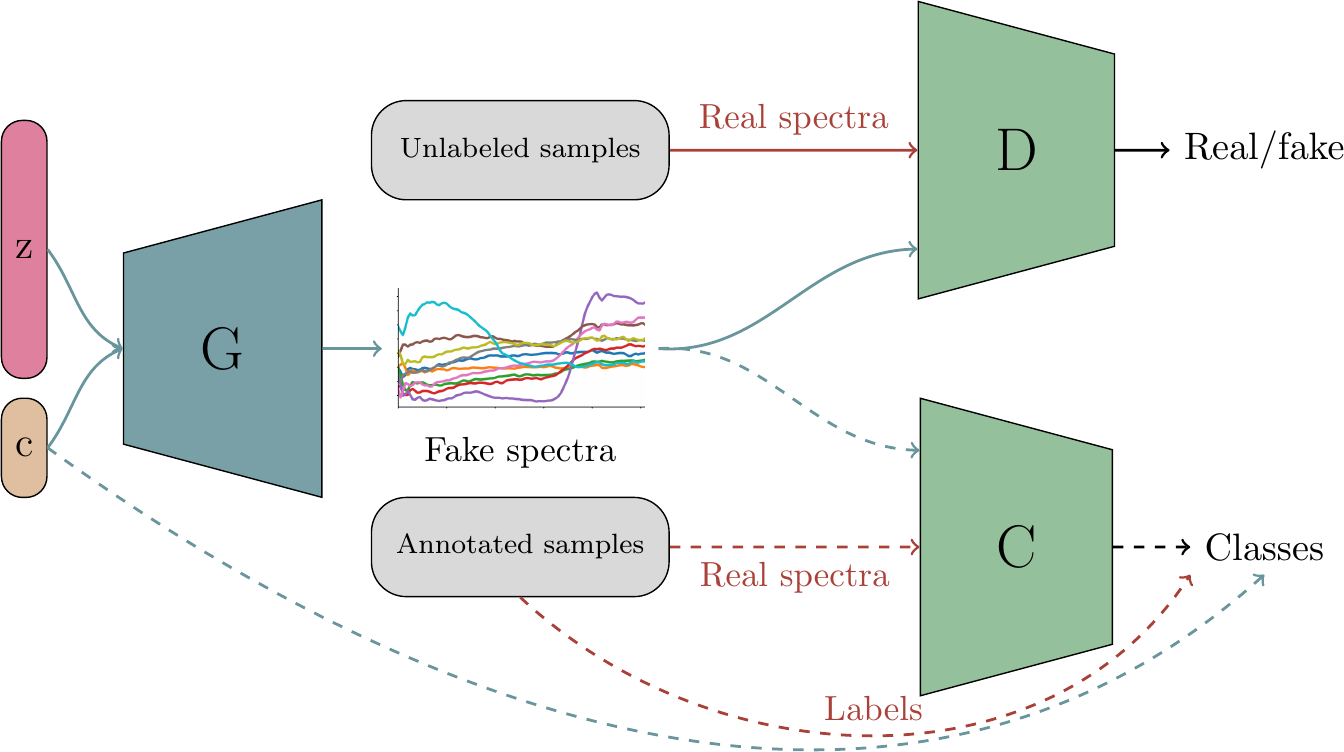
\includegraphics[width=\textwidth]{gan}
    \caption{La structure du \gls{GAN} utilisé pour la synthèse de spectres artificiels. Les flèches en \textcolor{BrickRed}{rouge} indiquent l'entraînement du classifieur et du discriminateur, tandis que les flèches en \textcolor{NavyBlue}{bleu} indiquent l'entraînement du générateur. Les flèches en pointillé indiquent les connexions qui ne sont utilisées que dans le cadre supervisé.}
    \label{fig:gan}
\end{figure}

Le principe des \gls{GAN} a été introduit par~\citet{goodfellow_generative_2014} en 2014. L'idée est d'utiliser des réseaux de neurones profonds pour approximer la distribution statistique sous-jacente à un ensemble d'observations. Un générateur est ainsi entraîner pour approximer la transformation entre un espace latent de bruit gaussien vers la distribution empirique observée. Cependant, la distribution n'est observée que sur quelques échantillons et l'on souhaite utiliser le générateur pour créer de nouveaux échantillons probables.Pour ce faire, le générateur est entraîné pour approximer la distribution à l'aide d'une fonction objectif adversaire. Cette fonction est implicitement définie en introduisant un second réseau, appelé discriminateur ou critique. Le discriminateur apprend à estimer si un échantillon donné provient de l'ensemble des données réelles ou bien a été généré artificiellement. À chaque étape de l'optimisation, le discriminateur est entraîné sur quelques itérations afin de lui permettre d'estimer la frontière entre données réelles et données synthétiques. Le générateur est ensuite optimisé de telle sorte à ce qu'il \emph{piège} le discriminateur, c'est-à-dire que les échantillons synthétisés soient indistinguables des exemples réels du point de vue du critique.

Plusieurs variantes du cadre des \gls{GAN} ont été proposées depuis leur introduction. Nous utilisons ici en particulier un générateur $G$ et un discriminateur $D$ utilisant le principe des Wasserstein \gls{GAN}~\cite{arjovsky_wasserstein_2017} utilisant la régularisation de~\citet{gulrajani_improved_2017}, dont l'entraînement est prévu pour minimiser la distance de Wasserstein entre la distribution réelle et la distribution synthétique. Toutefois, ce mode de fonctionnement est non-supervisé, c'est-à-dire qu'il n'est possible que de générer de nouveaux échantillons sans contrôle sur leur classe. Il serait possible de créer un générateur pour chaque classe, mais cela serait coûteux en temps et en mémoire. Dans notre cas, nous souhaitons pouvoir \emph{conditionner} le générateur par rapport à la classe du spectre que nous souhaitons synthétiser. Nous utilisons ainsi un classifieur auxiliaire $C$~\cite{odena_conditional_2017} qui ajoute une contrainte supplémentaire lors de l'optimisation du générateur en s'assurant que les spectres générés sont bien classifiés dans la classe choisie.
L'architecture complète est détaillée dans la~\cref{fig:gan}. Si $G$ et $D$ peuvent être entraînés sans annotation, c'est-à-dire de façon non-supervisée, $C$ nécessite des échantillons annotés pour être entraîné. L'ensemble est donc semi-supervisé et peut exploiter simultanément les échantillons annotés disponibles et le reste de l'image.

\section{Experimental setup}
\label{sec:experimental_setup}

Nous entraînons ce \gls{GAN} sur les jeux de données Pavia University, Pavia Center, Indian Pines et Botswana en utilisant les réflectances corrigées atmosphériquement lorsqu'elles sont disponibles. Comme nous essayons d'approximer des spectres individuels, nous utilisons pour $G$, $D$ et $C$ des réseaux simples entièrement connectés à 4 couches utilisant la fonction d'activation \emph{Leaky \gls{ReLU}}~\cite{maas_rectifier_2013}. La sortie de $G$ est suivie par une sigmoïde pour contraindre les valeurs de réflectance synthétisée entre $0$ et $1$. $D$ ne possède qu'une seule sortie et $C$ possède autant de sorties que le jeu de données a de classes.

L'optimisation des trois réseaux se fait en utilisant la politique de descente de gradient stochastique \emph{RMSProp}~\cite{rmsprop}. L'ensemble est entraîné durant 100 000 itérations avec une taille de \emph{batch} de 256, $C$ et $D$ étant entraînés 2 fois à chaque itération.

\section{Spectra analysis}
\label{sec:analysis}

Dans un premier temps, nous cherchons à comparer selon plusieurs critières les distributions synthétiques et réelles. Pour ce faire, nous entraînons d'abord deux \gls{GAN} sur Pavia University et Indian Pines.

\begin{figure}
\begin{subfigure}{0.5\textwidth}
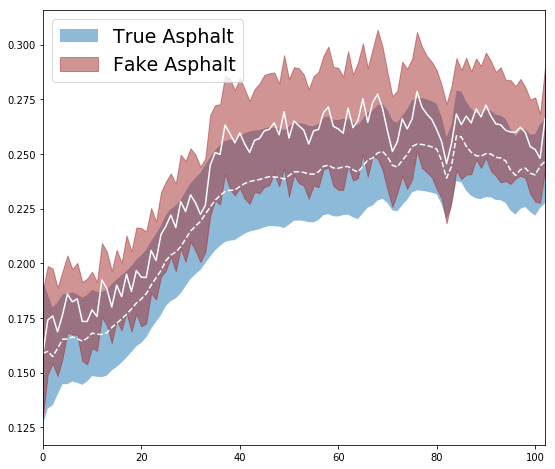
\includegraphics[width=\textwidth]{asphalt}
\end{subfigure}%
\begin{subfigure}{0.5\textwidth}
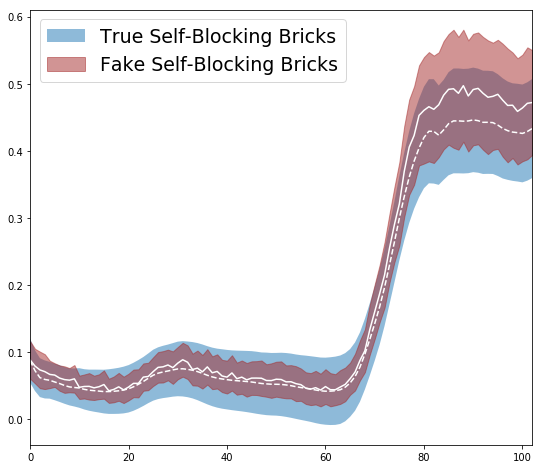
\includegraphics[width=\textwidth]{bricks}
\end{subfigure}
\caption{Spectre moyen et écart-type pour deux classes de matériaux du jeu de données Pavia Center. Les échantillons synthétiques moyens sont plus bruités et sont surappris sur certaines propriétés spectrales locales.}
\label{fig:mean_spectra}
\end{figure}

Visuellement, il est possible de constater dans la~\cref{fig:mean_spectra} que les spectres générés présentent des moments statistiques très similaires aux spectres réels. Les formes globales des spectres sont correctement approximés pour chaque classe. Toutefois, deux points négatifs sont identifiables. Tout d'abord, les spectres synthétiques moyens semblent plus bruités que leurs équivalents réels, ce qui signifie que le \gls{GAN} a surappris certaines particularités liées aux échantillons d'entraînement choisis. En outre, l'écart-type de la distribution synthétique est inférieur à celui de la distribution réelle, ce qui signifie que les faux spectres sont moins diversifiés que les vrais. Ces deux constatations indiquent que le générateur souffre partiellement d'une forme d'apprentissage appelée \emph{mode collapse}~\cite{salimans_improved_2016}.

\begin{figure}[t]
\begin{subfigure}{0.5\textwidth}
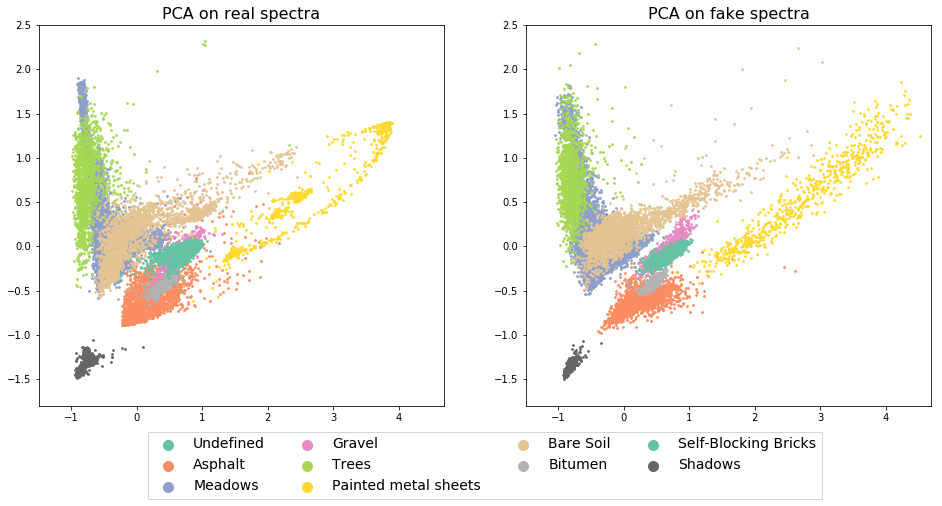
\includegraphics[width=\textwidth]{pca_paviau_acwgan}
\caption{Pavia University}
\end{subfigure}%
\begin{subfigure}{0.5\textwidth}
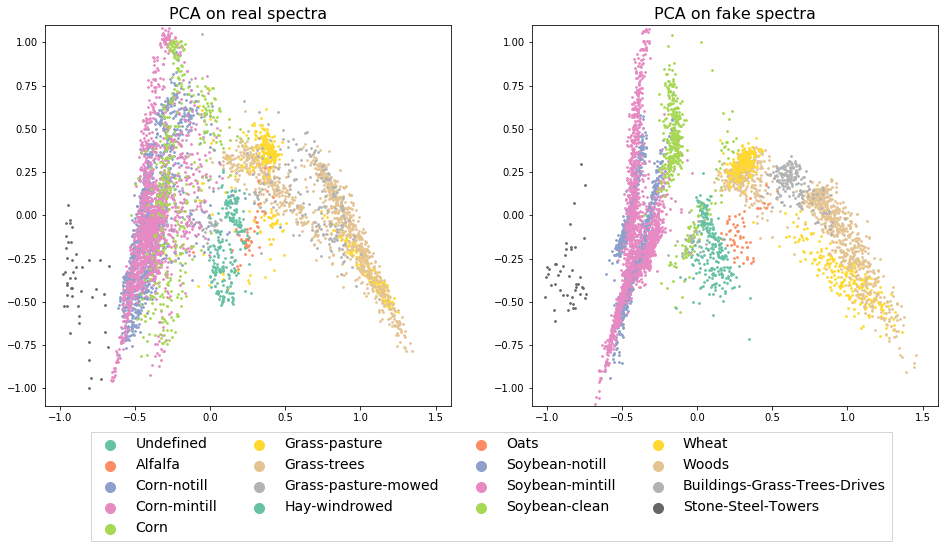
\includegraphics[width=\textwidth]{pca_indianpines_acwgan}
\caption{Indian Pines}
\end{subfigure}
\caption{\Gls{ACP} sur les spectres réels et synthétiques. Les spectres réels correspondent à l'ensemble des échantillons annotés de l'image. Les deux ensemble contiennent le même nombre d'éléments.}
\label{fig:pca}
\end{figure}

Pour mieux comprendre l'impact de ce surapprentissage, nous appliquons une \gls{ACP} afin de projeter les spectres réels et synthétiques dans un espace de représentation à deux dimensions (cf.~\cref{fig:pca}). Les groupes formés par les différentes classes sont correctement reproduits par les échantillons synthétiques. Cependant, la distribution synthétique présente également quelques déformations montrant que si le \gls{GAN} a bien réussi à modéliser la forme générale des différents types de spectres, il n'est cependant pas parvenu à reproduire l'ensemble de leurs spécificités.

\begin{table}[t]
	\begin{tabularx}{\textwidth}{c Y Y Y Y}
        Split & \multicolumn{2}{c}{Random (uniform)} & \multicolumn{2}{c}{Disjoint}\\
        \toprule
		\textbf{Train $\backslash$ Test} & Real & Fake & Real & Fake\\
        \midrule
        %\textbf{Train} & & & &\\
        Real & 89.5 & 98.3 & 87.2 & 98.8\\
        Fake & 87.8 & 99.2 & 79.4 & 99.9\\
        \bottomrule
	\end{tabularx}
    \caption{Exactitudes d'une \gls{SVM} linéaire appliquée sur les spectres réels et synthétiques du jeu de données Pavia University.}
    \label{table:svm_separation}
\end{table}

Nous pouvons essayer de construire une intuition sur la façon dont la distribution synthétique respecte les frontières entre classes de la distribution réelle en entraînant une \gls{SVM} linéaire sur les spectres réels et en l'appliquant pour séparer les spectres synthétiques. La \gls{SVM} va calculer les meilleurs hyperplans séparateurs pour la véritable distribution. Idéalement, ces hyperplans devraient séparer les spectres synthétiques exactement de la même façon. S'ils séparent nettement moins bien les spectres synthétiques, alors cela signifie que le générateur créé des échantillons irréalistes. S'ils séparent nettement mieux les échantillons, alors le générateur créé des exemples synthétiques trop similaires entre eux et regroupés autour des centroïdes corrsepondant aux classes réelles. Les résultats sont détaillés dans le~\cref{table:svm_separation}. Nous considérons deux approches\,: entraînement sur 3\% des spectres tirés au hasard uniformément ou sur 50\% de l'image, disjoint spatialement de la zone de validation. Dans le mode non-supervisé, nous utilisons également les échantillons non-annotés. Comme attendu, la \gls{SVM} sépare plus facilement les échantillons synthétiques que les spectres réels. Toutefois, entraîner la \gls{SVM} sur les spectres synthétiques uniquement permet tout de même de séparer les spectres réels dans une certaine mesure. Autrement dit, si les échantillons synthétiques sont moins diversifiés que les spectres réels, ils sont néanmoins représentatifs des différentes classes, et ce alors même que ces spectres sont générés \emph{ex nihilo} à partir de bruit aléatoire.

\begin{figure}[!t]
\begin{subfigure}{0.5\textwidth}
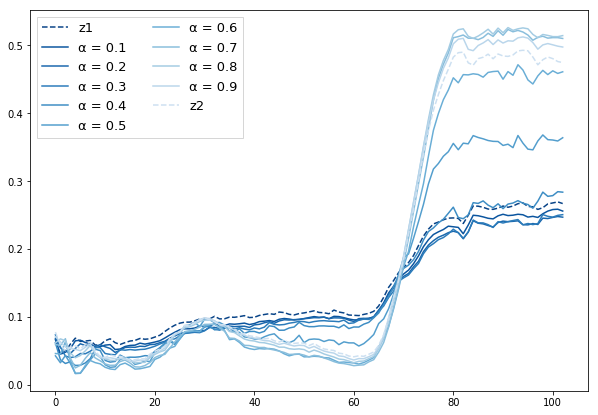
\includegraphics[width=0.95\textwidth]{interpolation_intraclass_acwgan}
\caption{Interpolation entre deux vecteurs latents de la classe ``sol nu''.}
\end{subfigure}%
\begin{subfigure}{0.5\textwidth}
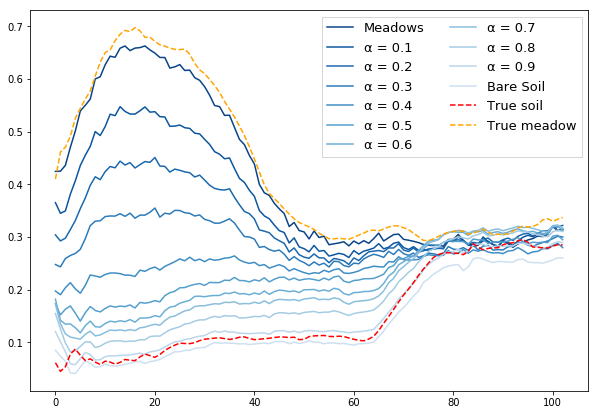
\includegraphics[width=0.95\textwidth]{interpolation_interclass_acwgan}
\caption{Interpolation à vecteur latent fixé entre les classes ``prairies'' et ``sol nu''.}
\end{subfigure}
\caption{Interpoler entre différents vecteurs ou conditionnements de l'espace latent permet d'explorer la variété des spectres de façon continue. Le \gls{GAN} est entraîné sur le jeu de données Pavia University. $\alpha$ contrôle l'interpolation.}
\label{fig:interpolation}
\end{figure}

Finalement, comme les \gls{GAN} permettent d'établir une projection entre un espace de représentation latent et le signal, il est possible d'explorer la variété des spectres en interpolant de façon continue entre deux points de l'espace latent. En particulier, il est également possible d'interpoler à vecteur de bruit fixe entre deux vecteurs de conditionnement. Ceci est illustré dans la~\cref{fig:interpolation}. Il existe une progression continue entre les échantillons générés, ce qui est particulièrement intéressant dans le cas de l'inteprolation entre classes. En effet, les spectres sont rarement purs et généralement constitués de mélanges, souvent non-linéaires, entre les réflectances de différents matériaux. Si les mélanges produits par le générateur sont réalistes, alors il effectue l'inverse de l'opération de démélange. Une approche d'apprentissage par dictionnaire, par inversion de modèle~\cite{gemp_inverting_2017} ou par plus proche voisin pourrait alors permettre, à partir d'un spectre réel soupçonné d'être un mélange, de revenir à ses \emph{endmembers} par une cartographie exhaustive de l'espace latent.

\begin{table*}[!t]
	\begin{tabularx}{\textwidth}{c c Y Y Y Y Y Y Y Y}
	\toprule
    \multicolumn{2}{c}{Dataset} & \multicolumn{2}{c}{PaviaU} & \multicolumn{2}{c}{PaviaC} & \multicolumn{2}{c}{Botswana} & \multicolumn{2}{c}{Indian Pines}\\
    Classifier & Augmentation & 3\% (r) & 50\% (s) & 3\% (r) & 50\% (s) & 3\% (r) & 50\% (s) & 3\% (r) & 50\% (s)\\
    \midrule
    \multirow{4}{*}{NN 1D} & $\emptyset$ & 92.72 & 86.22 & 98.93 & 96.26 & 86.90 & 84.87 & 79.44 & 74.00\\
    & GAN & 92.95 & 86.47 & 99.00 & 96.26 & 87.72 & 84.60 & 80.01 & 74.81\\
    & ss-GAN & 93.12 & 87.20 & 98.93 & 96.70 & 88.40 & 85.27 & 80.42 & 74.58\\
%     \midrule
%     \multirow{4}{*}{CNN 1D} & $\emptyset$ & - & - & - & - & - & - & - & -\\
%     & GAN & - & - & - & - & - & - & - & -\\
%     & ss-GAN & - & - & - & - & - & - & - & -\\
    \bottomrule
    \end{tabularx}
    \caption{Overall accuracies (OA) computed on several datasets with different data augmentation strategies. Sampling strategy is either a 50/50 spatial split of the image (s) or a uniform random sampling of 3\% of the labeled samples (r).}
    \label{table:da_results}
\end{table*}

\section{Data augmentation}
\label{sec:augmentation}

Les échantillons générés étant plausibles et représentatifs des spectres réels, nous suggérons de les utiliser pour enrichir les jeux de données annotés pré-existants. Nous testons cette idée sur plusieurs jeux de données : Indian Pines (aérien, rural), Pavia University (aérien, péri-urbain), Pavia Center (aérien, urbain) et Botswana (satellite, rural). Les résultats en mode supervisé et semi-supervisé sont détaillés dans le~\cref{table:da_results}. Augmenter le jeu de données à l'aide des faux spectres permet de légèrement augmenter les performances du classifieur.

Toutefois, augmenter drastiquement le nombre de faux spectres n'améliore pas plus la classification et finit même par la dégrader. En effet, dans ce cas les échantillons synthétiques deviennent prédominants dans la fonction de coût et dégradent les performances du classifieur, le ramenant vers le cas de la \gls{SVM} entraînée uniquement sur les faux spectres.

\section{Cas des données massives}

\subsection{Passage à l'échelle}

Supervisé mais large échelle

\todo[inline]{mini-france}

\todo[inline]{collab ESA}

%\bibliographystyle{plainnat}
%\bibliography{Chapitre5/Biblio}
\printbibliography
